\documentclass[../../thesis.tex]{subfiles}

\graphicspath{{./img/}}

\begin{document}

\subsection{Modifing the Activity driven network model}
\label{sec:modifing_activity_driven_model}



We pointed out the lack of memory on the general model proposed by \cite{perra2012activity} in Section~\ref{sec:activity_driven_model}. In this section we investigate a modification of the general model to support memory. We expect this change generates better motif distributions. We start by modifying the general activity driven model by adding a memory queue with fixed size $S$, following the \textit{First-In-First-Out} pattern on every node. Every node will have this queue which keeps track of who sent a transaction to him. In other words, the agents hold a record of from who they received Bitcoins. Figure~\ref{fig:proposed_model_queue_example} illustrates a temporal network with a memory queue of size $S=3$ on every node. The memory of Node 3 holds Node 1 at the head of the queue because the transaction T1 came first. Node 4 stores in its memory Node 3 at the head because the transaction T3 arrived early and Node 2 at the tail because the transaction T5 came later.


\begin{figure}
\centering
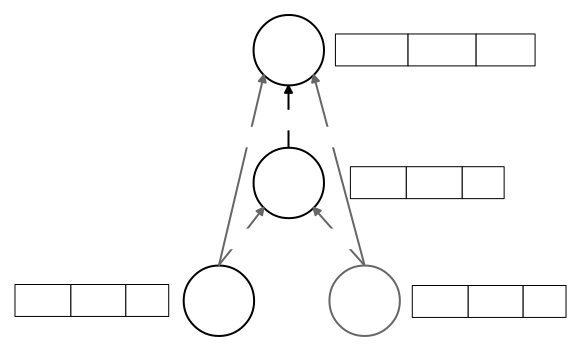
\includegraphics[width=0.8\textwidth]{content/modelling/img/proposed_model_queue_example}
\caption{Example of a temporal network with a memory queue on every node. In this figure, the memory queue has size $S=3$ and follows the First-In-First-Out pattern. Every node will have a queue which keeps track of receiver nodes. In other words, the agents hold a record of from who they got Bitcoins. The memory of Node 3 holds Node 1 at the head of the queue because the transaction T1 came first.  Node 4 store in its memory Node 3 at the head because the transaction T3 arrived early and Node 2 at the tail because the transaction T5 came later.}
\label{fig:proposed_model_queue_example}
\end{figure}

Our model has two phases at each time step where edges are generated. The first phase is the activity driven edge generation described in the previous section, and the second phase is edge generation from the memory pool. During this phase, every node with a non-empty memory pool generates an edge to each of the nodes stored in its memory pool. This simulates persistance. Additionally, we set the current runtime timestamp in seconds as time value of the generated temporal edges. For simplicity, we will call this modified model "model A".

%Figure \ref{fig:proposed_activity_driven_model_with_money} represents a simulation example in 3-time steps of the above proposed model. Step $T=1$, only active nodes make connections, is the first interaction. Consequently, the memory queues are empty. Step $T=2$ two nodes are memory active and transfer back the funds to node origin. Finally, at Step $T=3$, only one node is memory active, this node was on hold since the previous steps.


%Generally, our proposed model will try to capture the natural common sense of Bitcoins agents. Agents have a higher probability of engaging again in a trade with past involved nodes. 



%\begin{figure}[H]
%\centering
%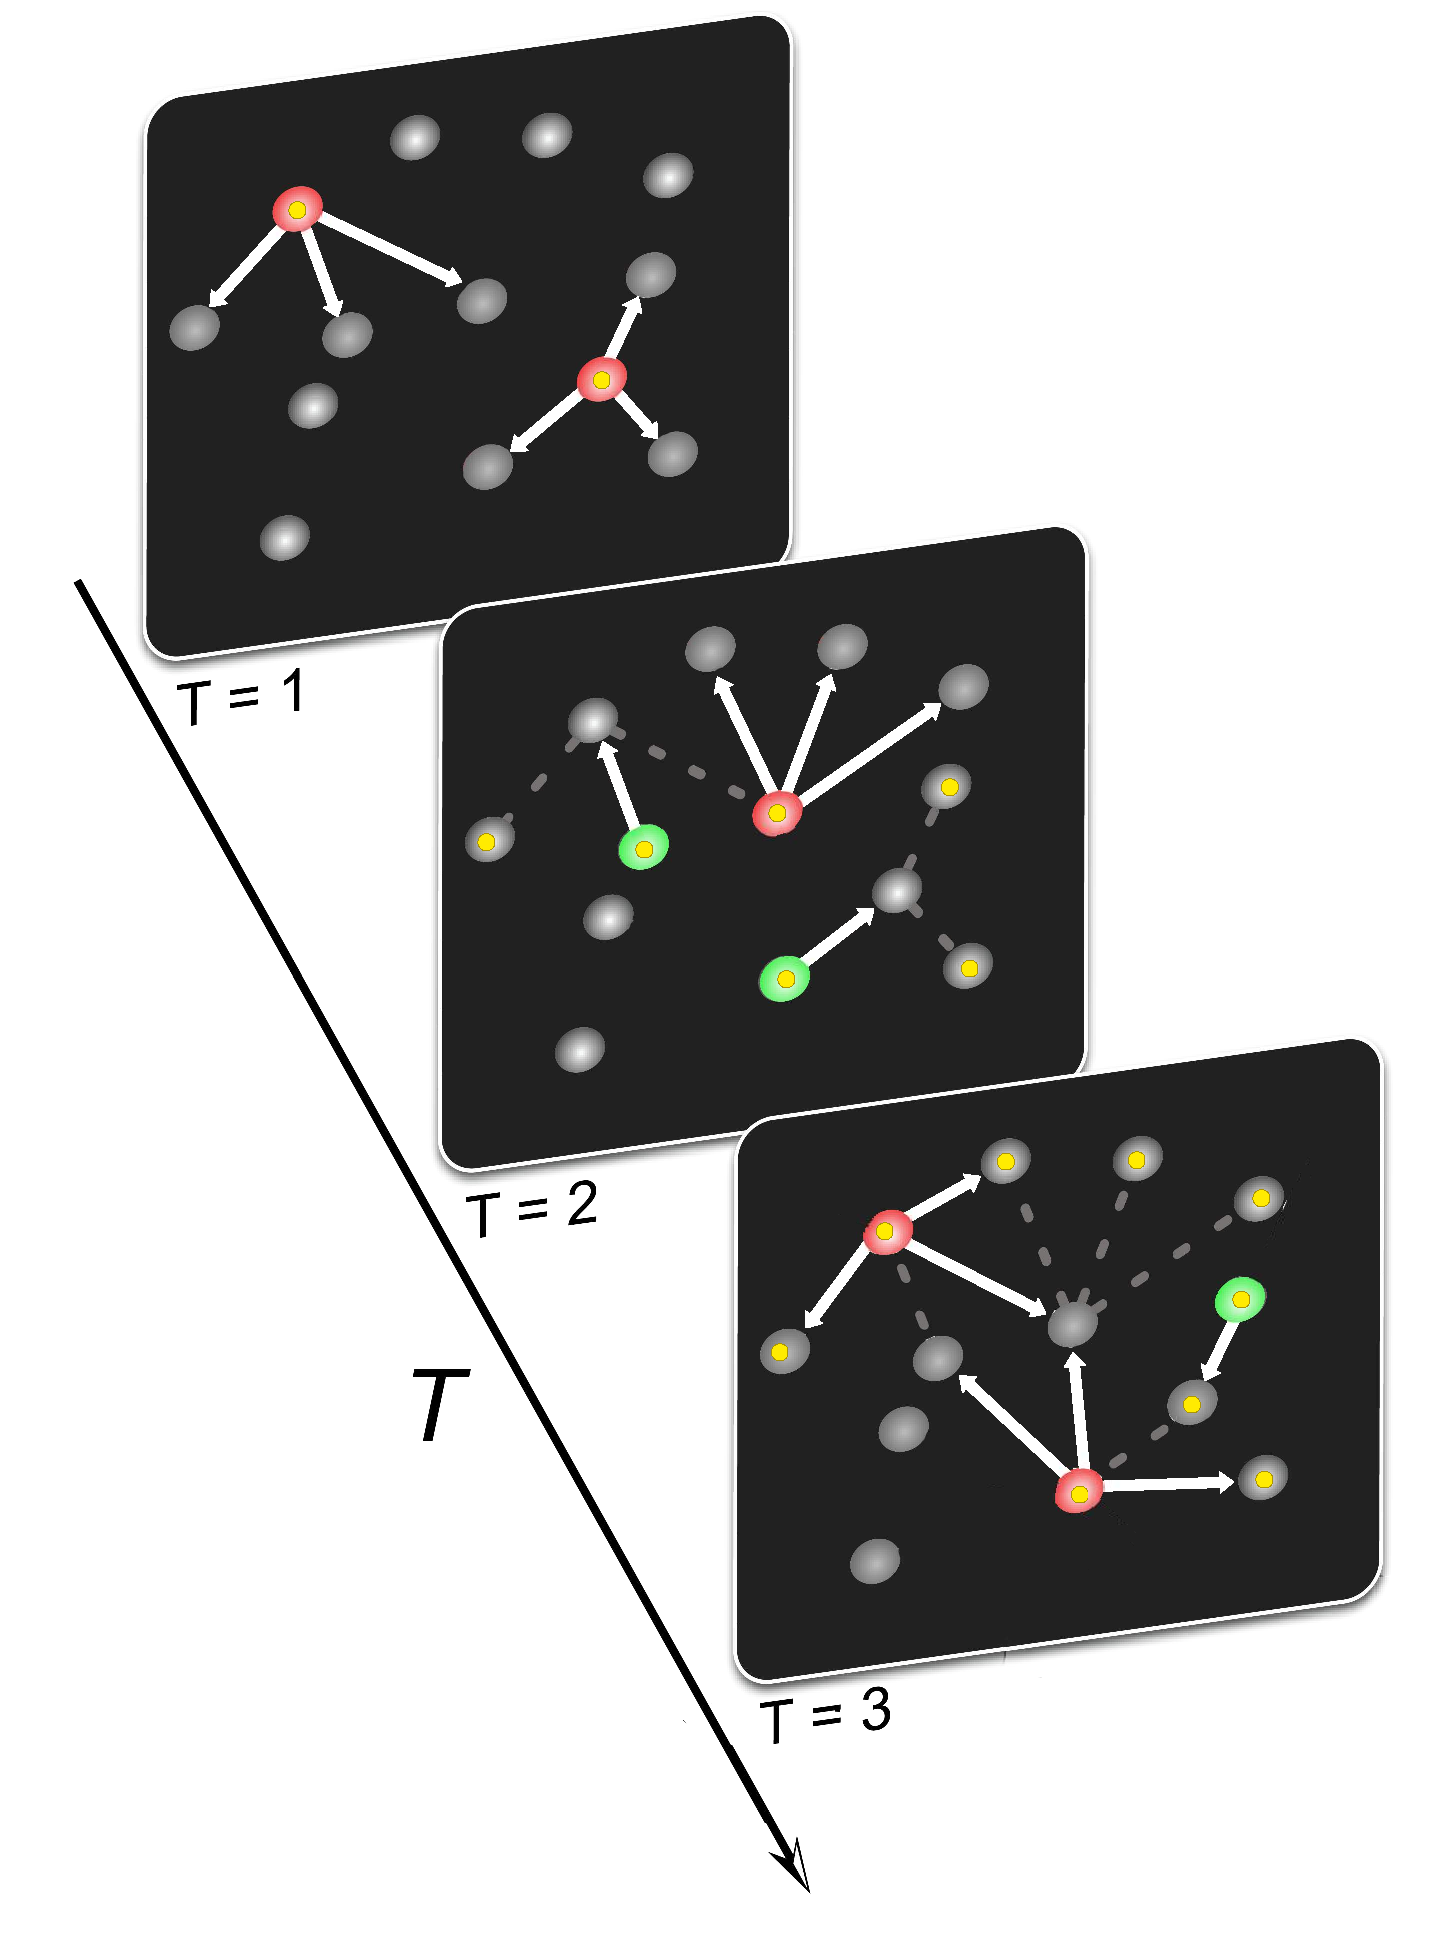
\includegraphics[width=0.8\textwidth]{content/modelling/img/proposed_activity_driven_model_with_money}
%\caption{Graphical representation of a simulation running proposed model running in 3-time steps with activity connections $m=3$; memory connections $s=1$; number of nodes $N=13$. Red color indicates active nodes; green represents memory active nodes; grey illustrates not active nodes; small yellow circle represents units of money. Dashed lines show past connections. Step $T=1$, only active nodes make connections, is the first interaction. Consequently, the memory queues are empty. Step $T=2$ two nodes are memory active and transfer back the funds to node origin. Finally, at Step $T=3$, only one node is memory active, this node was on hold since the previous steps.}
%\label{fig:proposed_activity_driven_model_with_money}
%\end{figure}





\end{document}


